\section{Шифрование блока}\label{BLOCK}

\subsection{Интерфейс}\label{BLOCK.IFace}

Шифрование блока задается алгоритмами зашифрования~$\algname{belt-block}$
и расшифрования~$\algname{belt-block}^{-1}$.

Входными данными~$\algname{belt-block}$ являются блок~$X\in\{0,1\}^{128}$ 
и ключ~$K\in\{0,1\}^{256}$. 
%
Выходными данными является зашифрованный блок~$Y\in\{0,1\}^{128}$.

Входными данными~$\algname{belt-block}^{-1}$ являются зашифрованный 
блок~$Y\in\{0,1\}^{128}$ и ключ~$K\in\{0,1\}^{256}$. 
%
Выходными данными является расшифрованный блок~$X\in\{0,1\}^{128}$.

\subsection{Вспомогательные преобразования и переменные}\label{BLOCK.Aux} 

\begin{table}[bht]
\caption{Подстановка~$H$}\label{Table.SBOX}
{\small\tt
{\tabcolsep=8.5pt
\begin{tabular}{|l|rrrrrrrrrrrrrrrr|}
\hline
 &  0&  1&  2&  3&  4&  5&  6&  7&  8&  9&  A&  B&  C&  D&  E&  F\\
\hline
0& B1& 94& BA& C8& 0A& 08& F5& 3B& 36& 6D& 00& 8E& 58& 4A& 5D& E4\\
1& 85& 04& FA& 9D& 1B& B6& C7& AC& 25& 2E& 72& C2& 02& FD& CE& 0D\\
2& 5B& E3& D6& 12& 17& B9& 61& 81& FE& 67& 86& AD& 71& 6B& 89& 0B\\
3& 5C& B0& C0& FF& 33& C3& 56& B8& 35& C4& 05& AE& D8& E0& 7F& 99\\
4& E1& 2B& DC& 1A& E2& 82& 57& EC& 70& 3F& CC& F0& 95& EE& 8D& F1\\
5& C1& AB& 76& 38& 9F& E6& 78& CA& F7& C6& F8& 60& D5& BB& 9C& 4F\\
6& F3& 3C& 65& 7B& 63& 7C& 30& 6A& DD& 4E& A7& 79& 9E& B2& 3D& 31\\
7& 3E& 98& B5& 6E& 27& D3& BC& CF& 59& 1E& 18& 1F& 4C& 5A& B7& 93\\
8& E9& DE& E7& 2C& 8F& 0C& 0F& A6& 2D& DB& 49& F4& 6F& 73& 96& 47\\
9& 06& 07& 53& 16& ED& 24& 7A& 37& 39& CB& A3& 83& 03& A9& 8B& F6\\
A& 92& BD& 9B& 1C& E5& D1& 41& 01& 54& 45& FB& C9& 5E& 4D& 0E& F2\\
B& 68& 20& 80& AA& 22& 7D& 64& 2F& 26& 87& F9& 34& 90& 40& 55& 11\\
C& BE& 32& 97& 13& 43& FC& 9A& 48& A0& 2A& 88& 5F& 19& 4B& 09& A1\\
D& 7E& CD& A4& D0& 15& 44& AF& 8C& A5& 84& 50& BF& 66& D2& E8& 8A\\
E& A2& D7& 46& 52& 42& A8& DF& B3& 69& 74& C5& 51& EB& 23& 29& 21\\
F& D4& EF& D9& B4& 3A& 62& 28& 75& 91& 14& 10& EA& 77& 6C& DA& 1D\\
\hline
\end{tabular}
} % tabcolsep
} % tt
\end{table}

\paragraph{Подстановка $H$.}
Подстановка $H\colon\{0,1\}^8\to\{0,1\}^8$ задается
таблицей~\ref{Table.SBOX}.
%
В таблице входы (прообразы) и выходы (образы) $H$ записываются в 
шестнадцатеричном виде.
%
Для входного октета $u=\hex{IJ}$ соответствующий выходной октет~$H(u)$ 
находится на пересечении строки $\hexz{I}$ и столбца~$\hexz{J}$. 
Например, $H(\hex{A2})=\hex{9B}$.

\paragraph{Преобразования $G_r$ ($r=5,13,21$).}
Преобразование $G_r\colon\{0,1\}^{32}\to\{0,1\}^{32}$
ставит в соответствие слову
$u=u_1\parallel u_2\parallel u_3\parallel u_4$,
$u_i\in\{0,1\}^8$,
слово
$$
G_r(u)=\RotHi^r\left(
H(u_1)\parallel H(u_2)\parallel H(u_3)\parallel H(u_4)
\right).
$$

\paragraph{Переменные.}
Используются переменные~$a,b,c,d,e\in\{0,1\}^{32}$.

\subsection{Алгоритм зашифрования}\label{BLOCK.Encr}

Зашифрование~$\algname{belt-block}(X,K)$ выполняется следующим
образом: 
\begin{enumerate}
\item
Определить $(X_1,X_2,X_3,X_4)=\Split(X,32)$.
\item
Определить $(K_1,K_2,\ldots,K_8)=\Split(K,32)$.
\item
Обозначить $k[i]=K_{(i-1)\bmod 8 + 1}$, $i=1,2,\ldots,56$.
\item
Установить $a\leftarrow X_1$, $b\leftarrow X_2$, 
$c\leftarrow X_3$, $d\leftarrow X_4$.
\item
Для $i=1,2,\ldots,8$ выполнить (см.~рисунок~\ref{Figure.BLOCK.Round}):
\begin{enumerate}
\item
$b\leftarrow b\oplus G_{5}(a\boxplus k[7i-6])$;
\item
$c\leftarrow c\oplus G_{21}(d\boxplus k[7i-5])$;
\item
$a\leftarrow a\boxminus G_{13}(b\boxplus k[7i-4])$;
\item
$e\leftarrow G_{21}(b\boxplus c\boxplus k[7i-3])\oplus
\itob{i}_{32}$;
\item
$b\leftarrow b\boxplus  e$;
\item
$c\leftarrow c\boxminus e$;
\item
$d\leftarrow d\boxplus G_{13}(c\boxplus k[7i-2])$;
\item
$b\leftarrow b\oplus G_{21}(a\boxplus k[(7i-1])$;
\item
$c\leftarrow c\oplus G_{5}(d\boxplus k[7i])$;
\item
$a\leftrightarrow b$;
\item
$c\leftrightarrow d$;
\item
$b\leftrightarrow c$.
\end{enumerate}
\item
Установить~$Y\leftarrow b\parallel d\parallel a\parallel c$.
\item
Возвратить $Y$.
\end{enumerate}

\begin{figure}[bht]
\begin{center}
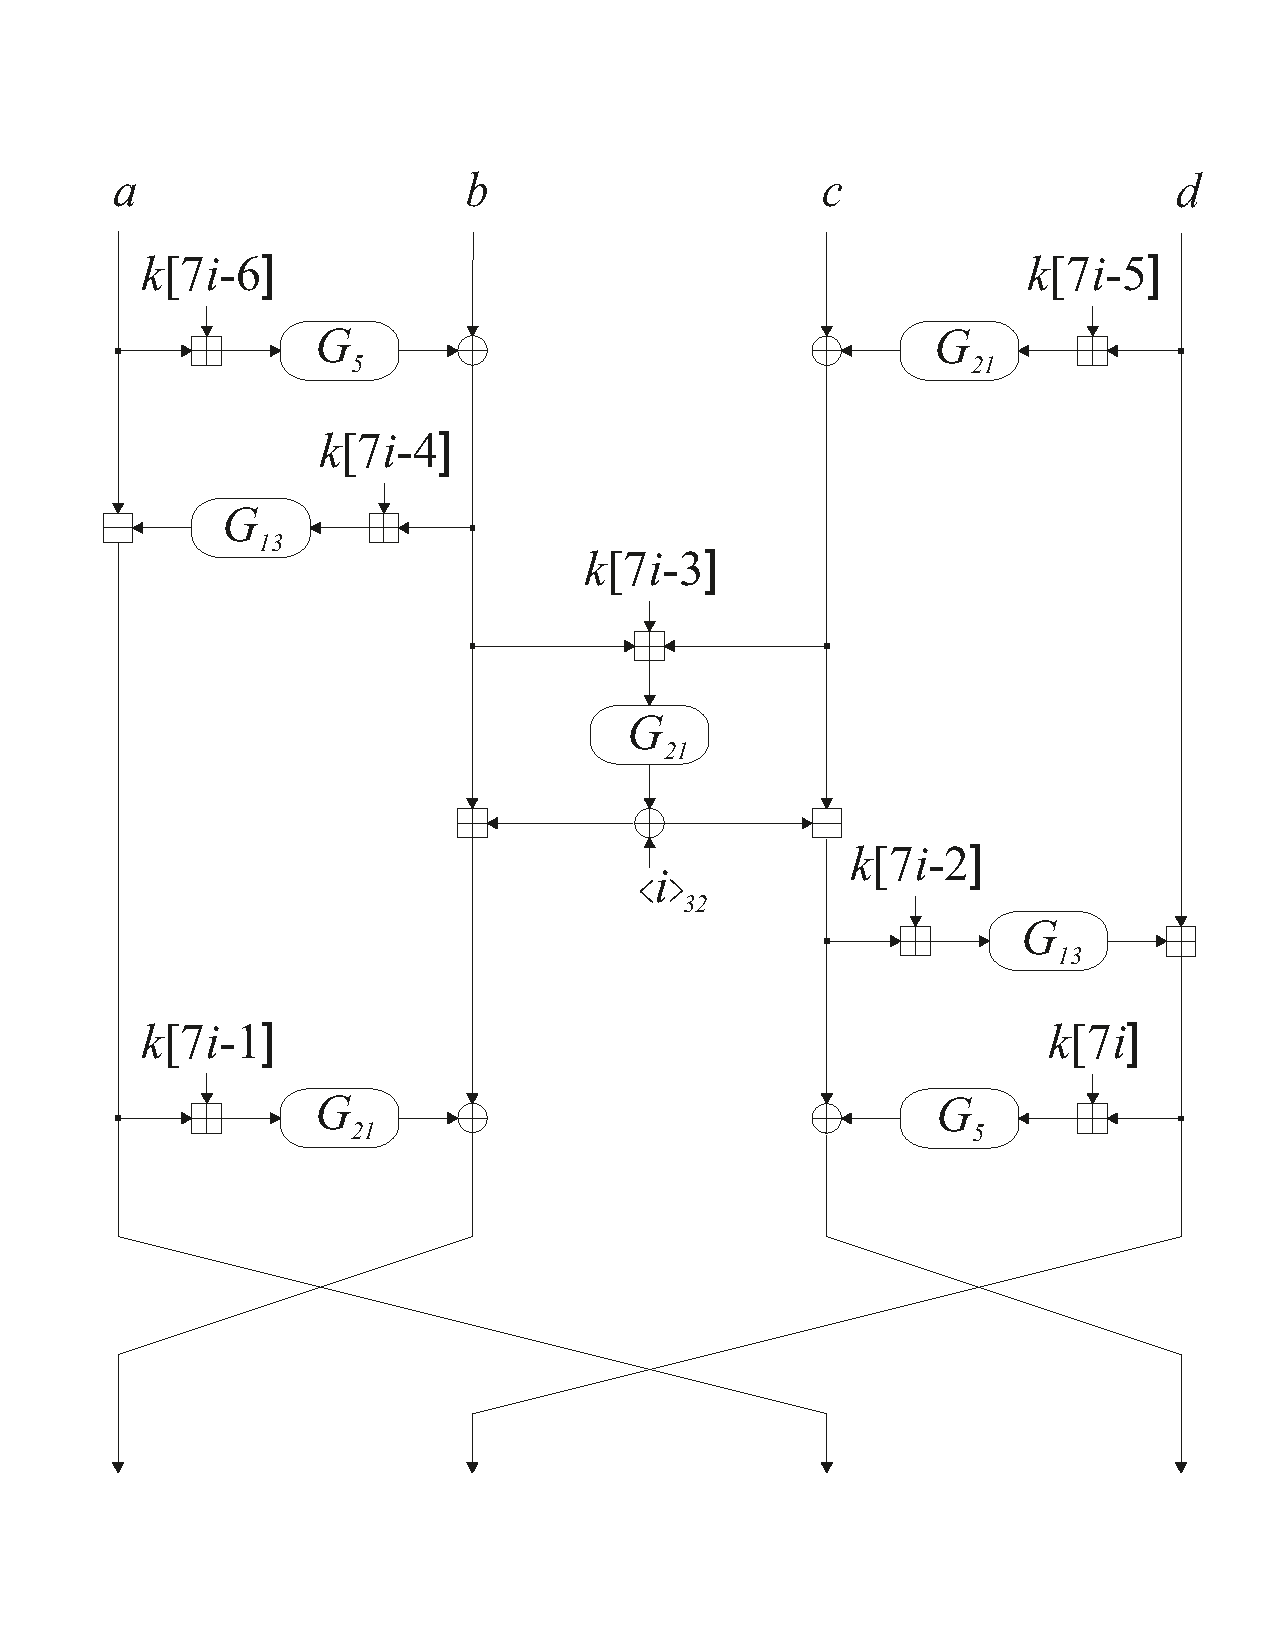
\includegraphics[width=10cm]{../figs/belt-round}
\end{center}
\caption{Вычисления на $i$-м такте зашифрования}\label{Figure.BLOCK.Round}
\end{figure}

\subsection{Алгоритм расшифрования}\label{BLOCK.Decr}

Расшифрование~$\algname{belt-block}^{-1}(Y,K)$ выполняется
следующим образом: 
\begin{enumerate}
\item
Определить $(Y_1,Y_2,Y_3,Y_4)=\Split(Y,32)$.
\item
Определить $(K_1,K_2,\ldots,K_8)=\Split(K,32)$.
\item
Обозначить $k[i]=K_{(i-1)\bmod 8 + 1}$, $i=1,2,\ldots,56$.
\item
Установить $a\leftarrow Y_1$, $b\leftarrow Y_2$, 
$c\leftarrow Y_3$, $d\leftarrow Y_4$.
\item
Для $i=8,7,\ldots,1$ выполнить:
\begin{enumerate}
\item
$b\leftarrow b\oplus G_{5}(a\boxplus k[7i])$;
\item
$c\leftarrow c\oplus G_{21}(d\boxplus k[7i-1])$;
\item
$a\leftarrow a\boxminus G_{13}(b\boxplus k[7i-2])$;
\item
$e\leftarrow G_{21}(b\boxplus c\boxplus k[7i-3])\oplus \itob{i}_{32}$;
\item
$b\leftarrow b\boxplus e$;
\item
$c\leftarrow c\boxminus e$;
\item
$d\leftarrow d\boxplus G_{13}(c\boxplus k[7i-4])$;
\item
$b\leftarrow b\oplus G_{21}(a\boxplus k[7i-5])$;
\item
$c\leftarrow c\oplus G_{5}(d\boxplus k[7i-6])$;
\item
$a\leftrightarrow b$;
\item
$c\leftrightarrow d$;
\item
$a\leftrightarrow d$.
\end{enumerate}
\item
Установить~$X\leftarrow c\parallel a\parallel d\parallel b$.
\item
Возвратить $X$.
\end{enumerate}
